%%%%%%%%%%%%%%%%%%%%%%%%%%%%%%%%%%%%%%%%%
% Beamer Presentation
% LaTeX Template
% Version 1.0 (10/11/12)
%
% This template has been downloaded from:
% http://www.LaTeXTemplates.com
%
% License:
% CC BY-NC-SA 3.0 (http://creativecommons.org/licenses/by-nc-sa/3.0/)
%
%%%%%%%%%%%%%%%%%%%%%%%%%%%%%%%%%%%%%%%%%

%----------------------------------------------------------------------------------------
%	PACKAGES AND THEMES
%----------------------------------------------------------------------------------------

\documentclass{beamer}

\mode<presentation> {

% The Beamer class comes with a number of default slide themes
% which change the colors and layouts of slides. Below this is a list
% of all the themes, uncomment each in turn to see what they look like.

%\usetheme{default}
%\usetheme{AnnArbor}
%\usetheme{Antibes}
%\usetheme{Bergen}
%\usetheme{Berkeley}
%\usetheme{Berlin}
%\usetheme{Boadilla}
%\usetheme{CambridgeUS}
%\usetheme{Copenhagen}
\usetheme{Darmstadt}
%\usetheme{Dresden}
%\usetheme{Frankfurt}
%\usetheme{Goettingen}
%\usetheme{Hannover}
%\usetheme{Ilmenau}
%\usetheme{JuanLesPins}
%\usetheme{Luebeck}
%\usetheme{Madrid}
%*\usetheme{Malmoe}
%\usetheme{Marburg}
%\usetheme{Montpellier}
%\usetheme{PaloAlto}
%\usetheme{Pittsburgh}
%\usetheme{Rochester}
%\usetheme{Singapore}
%\usetheme{Szeged}
%\usetheme{Warsaw}

% As well as themes, the Beamer class has a number of color themes
% for any slide theme. Uncomment each of these in turn to see how it
% changes the colors of your current slide theme.

%\usecolortheme{albatross}
%\usecolortheme{beaver}
%\usecolortheme{beetle}
%\usecolortheme{crane}
%\usecolortheme{dolphin}
%\usecolortheme{dove}
%\usecolortheme{fly}
%\usecolortheme{lily}
\usecolortheme{orchid}
%\usecolortheme{rose}
%\usecolortheme{seagull}
%\usecolortheme{seahorse}
%\usecolortheme{whale}
%\usecolortheme{wolverine}

%\setbeamertemplate{footline} % To remove the footer line in all slides uncomment this line
%\setbeamertemplate{footline}[page number] % To replace the footer line in all slides with a simple slide count uncomment this line

%\setbeamertemplate{navigation symbols}{} % To remove the navigation symbols from the bottom of all slides uncomment this line
}


\usepackage{graphicx} % Allows including images
\usepackage{booktabs} % Allows the use of \toprule, \midrule and \bottomrule in tables
\usepackage{xspace}
\usepackage{caption}
\usepackage{subfigure}
\usepackage[english,brazil]{babel}
\usepackage[utf8]{inputenc}

%Renomeia o nome padrao das figuras.
\renewcommand{\figurename}{Figura}
\renewcommand{\tablename}{Tabela}
%----------------------------------------------------------------------------------------
%	TITLE PAGE
%----------------------------------------------------------------------------------------

\title[Computação Gráfica]{Introdução à Computação Gráfica} % The short title appears at the bottom of every slide, the full title is only on the title page

\author{Uéliton Freitas} % Your name
\institute[UFMS] % Your institution as it will appear on the bottom of every slide, may be shorthand to save space
{
Universidade Católica Don Bosco - UCDB \\ % Your institution for the title page
\medskip
\textit{freitas.ueliton@gmail.com} % Your email address
}
\date{\today} % Date, can be changed to a custom date


\begin{document}

\begin{frame}
\titlepage % Print the title page as the first slide
\end{frame}

\begin{frame}
\frametitle{Sumário} % Table of contents slide, comment this block out to remove it
\tableofcontents % Throughout your presentation, if you choose to use \section{} and \subsection{} commands, these will automatically be printed on this slide as an overview of your presentation
\end{frame}




%----------------------------------------------------------------------------------------
%	PRESENTATION SLIDES
%----------------------------------------------------------------------------------------

%------------------------------------------------
\section{Introdução} 
%------------------------------------------------

%\section{Speeded-Up Robust Features - SURF} % A subsection can be created just before a set of slides with a common theme to further break down your presentation into chunks
%\section{Baf Of Features and Colors}

%\section{Refer\^encias}
%%%%%%%%%%%%%%%%%%%%%%%%%%%%%%%%%%%%%%%%%%%%%%%%%%%%%%%%%%%%%%%%%%%%%%%%%%%%%%%%%%%%%%%%%%
\begin{frame}
\frametitle{Introdução}


	\begin{block}{O que será revisto?}
		\begin{itemize}
			\item Notações dos elementos.
			\item Conjuntos.
			\item Funções.
		\end{itemize}
	\end{block}
	
\end{frame}


%%%%%%%%%%%%%%%%%%%%%%%%%%%%%%%%%%%%%%%%%%%%%%%%%%%%%%%%%%%%%%%%%%%%%%%%%%%%%%%%%%%%%%%%%%
\section{Notações}
\begin{frame}
\frametitle{Notações}


	\begin{block}{Notações Matemáticas Convencionais}
		\begin{itemize}
			\item<1-> A maioria das variáveis estarão em \textit{itálico}: \textit{x,y}.
			\item<2-> Vetores estarão em negrito e em letras romanas: \textbf{u}.
			\item<3-> Matrizes estarão em letras romanas, negrito e em caixa alta:\textbf{A}.
			\item<4-> Algumas letras são utilizadas para denotar alguns conjuntos como:
				\begin{itemize}
					\item $\mathbb{R}$: Números Reais.
					\item $\mathbb{R}^+$: Números Reais Positivos.
					\item $\mathbb{R}_0^+$: Números Reais \textbf{não} negativos.
				\end{itemize}
		\end{itemize}
	
	\end{block}
	
\end{frame}


%%%%%%%%%%%%%%%%%%%%%%%%%%%%%%%%%%%%%%%%%%%%%%%%%%%%%%%%%%%%%%%%%%%%%%%%%%%%%%%%%%%%%%%%%%
\section{Conjuntos}
\subsection{Notações}
\begin{frame}
\frametitle{Conjuntos}


	\begin{block}{Notações Matemáticas Convencionais}
		\begin{itemize}
			\item<1-> Conjuntos são denotados por letras maiúsculas: B.
			\item<2-> O produto cartesiano de dos conjuntos B $\times$ C é denotado por:
				\begin{itemize}
					\item $ B \times C = \{(b,c) : b \in B ,  c \in C\}$
					\item Conjuntos de todos os pares ordenados $(b,c)$ tal que  $b \in B$ e $c \in C$.
				\end{itemize}
			\item<3-> O produto de $\mathbb{R} \times \mathbb{R}$ é denotado por $\mathbb{R}^2$.
			\item<4-> Produtos de alta ordem de $\mathbb{R}$ são denotados por $\mathbb{R}^2$,$\mathbb{R}^3$,$\mathbb{R}^4$,...
		\end{itemize}
	\end{block}
	
\end{frame}

%%%%%%%%%%%%%%%%%%%%%%%%%%%%%%%%%%%%%%%%%%%%%%%%%%%%%%%%%%%%%%%%%%%%%%%%%%%%%%%%%%%%%%%%%%
\subsection{Intervalos}
\begin{frame}
\frametitle{Conjuntos}


	\begin{block}{Intervalos}
		\begin{itemize}
			\item<1-> O intervalo fechado $[a,b] \in \mathbb{R}$ é o conjunto de todos os números reais entre $a$ e $b$ incluindo os mesmos.
			\begin{itemize}
				\item $[a,b] = \{ x : a \leq x \leq b \}$
			\end{itemize}
			
			\item<2-> O intervalo semi aberto $(a,b],[a,b) \in \mathbb{R}$ é o conjunto de todos os números reais entre $a$ e $b$, que \textbf{podem} ou \textbf{não} incluir os mesmos.
			\begin{itemize}
				\item $(a,b] = \{ x : a < x \leq b \}$
				\item $[a,b) = \{ x : a \leq x < b \}$
			\end{itemize}
			
			\item<3-> O intervalo aberto $(a,b) \in \mathbb{R}$ é o conjunto de todos os números reais entre $a$ e $b$, que \textbf{não} incluem os mesmos.
			\begin{itemize}
				\item $(a,b) = \{ x : a < x < b \}$
			\end{itemize}
		\end{itemize}
	\end{block}
	
\end{frame}


%%%%%%%%%%%%%%%%%%%%%%%%%%%%%%%%%%%%%%%%%%%%%%%%%%%%%%%%%%%%%%%%%%%%%%%%%%%%%%%%%%%%%%%%%%
\begin{frame}
\frametitle{Conjuntos}


	\begin{block}{Notações Matemáticas Convencionais}
		\begin{itemize}
			\item Outras convenções de intervalos:
				\begin{itemize}
					\item<1-> Intervalo de $a$(inclusive) até mais infinito:\\$[a,\infty) = \{ x : a \leq \infty \}$
					\item<2-> Intervalo de $-\infty$ até $b$(inclusive):\\$(-\infty,b] = \{ x : -\infty \leq b \}$
				\end{itemize}
		\end{itemize}
	\end{block}
	
\end{frame}

%%%%%%%%%%%%%%%%%%%%%%%%%%%%%%%%%%%%%%%%%%%%%%%%%%%%%%%%%%%%%%%%%%%%%%%%%%%%%%%%%%%%%%%%%%
\section{Funções}
\subsection{Notação de uma Função}
\begin{frame}
\frametitle{Funções}

	\begin{block}{Notação de uma Função}
		\begin{itemize}
			\item<1-> Uma função $f$ é denotada da seguinte forma:
				\begin{itemize}
					\item $f:\mathbb{R} \to \mathbb{R} : x \mapsto x^2$
				\end{itemize}
			\item<2-> O nome da função é $f$.
			\item<3-> O elemento do lado esquerdo da seta($\mapsto$) é denominado \textbf{Domínio}.
			\item<4-> O elemento do lado direito da seta($\mapsto$) é denominado \textbf{Imagem} ou \textbf{Codomínio}.
		\end{itemize}
	\end{block}
	
\end{frame}

%%%%%%%%%%%%%%%%%%%%%%%%%%%%%%%%%%%%%%%%%%%%%%%%%%%%%%%%%%%%%%%%%%%%%%%%%%%%%%%%%%%%%%%%%%
\subsection{Funções Injetoras}

\begin{frame}
\frametitle{Funções}

	\begin{block}{Funções Injetoras}
		\begin{itemize}
			\item Seja a função $g: A \to B$.
			\item<1-> Dizemos que uma função $g$ é \textbf{injetora} se $ \forall a_1,a_2 \in A, g(a_1) \neq g(a_2) \in B$.
		\end{itemize}
	\end{block}
	
	\begin{figure}[!h]
			\begin{center}
			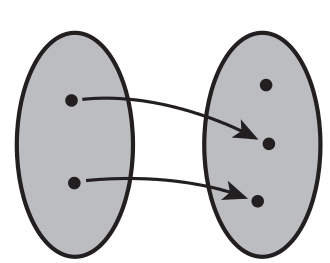
\includegraphics[width=0.5\textwidth]{Figures/injetora}
			\end{center}
	\end{figure}	
	
\end{frame}

%%%%%%%%%%%%%%%%%%%%%%%%%%%%%%%%%%%%%%%%%%%%%%%%%%%%%%%%%%%%%%%%%%%%%%%%%%%%%%%%%%%%%%%%%%

\begin{frame}
\frametitle{Funções}

	\begin{block}{Funções Injetoras}
		\begin{itemize}
			\item<1-> Dizemos que uma função $g$ é \textbf{injetora} se $ \forall x_1,x_2 \in A, g(x_1) \neq g(x_2) \in B$.
		\end{itemize}
	\end{block}
	
	\begin{block}{Exemplo de uma Função Injetora}
		\begin{itemize}
			\item Seja a função: $g: \mathbb{R} \to \mathbb{R}_0^+ : g(x) = x^2$
		\end{itemize}
	\end{block}
	\begin{figure}[!h]
			\begin{center}
			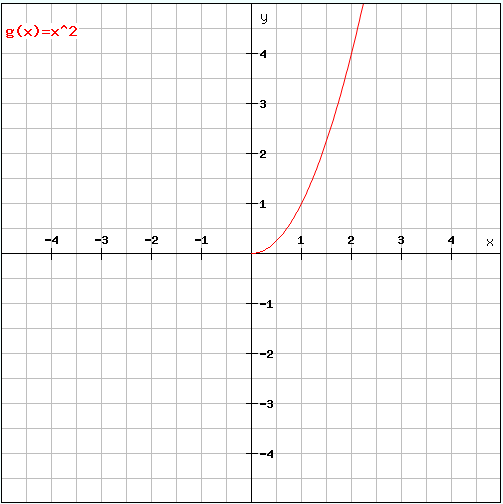
\includegraphics[width=0.35\textwidth]{Figures/g}
			\end{center}
	\end{figure}	
	
\end{frame}


%%%%%%%%%%%%%%%%%%%%%%%%%%%%%%%%%%%%%%%%%%%%%%%%%%%%%%%%%%%%%%%%%%%%%%%%%%%%%%%%%%%%%%%%%%
\subsection{Funções Sobrejetoras}

\begin{frame}
\frametitle{Funções}

	\begin{block}{Funções Sobrejetoras}
		\begin{itemize}
			\item Seja a função $f: A \to B$.
			\item<1-> Dizemos que uma função $f$ é \textbf{sobrejetora} se, e somete se:\\ $ \forall b \in B,\exists a \in A : b = f(a)$.
		\end{itemize}
	\end{block}
	
	\begin{figure}[!h]
			\begin{center}
			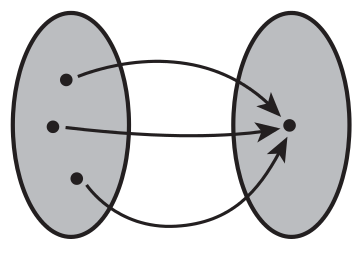
\includegraphics[width=0.5\textwidth]{Figures/sobrejetora}
			\end{center}
	\end{figure}	
	
\end{frame}

%%%%%%%%%%%%%%%%%%%%%%%%%%%%%%%%%%%%%%%%%%%%%%%%%%%%%%%%%%%%%%%%%%%%%%%%%%%%%%%%%%%%%%%%%%

\begin{frame}
\frametitle{Funções}

	\begin{block}{Funções Sobrejetora}
		\begin{itemize}
			\item<1-> Dizemos que uma função $f$ é \textbf{sobrejetora} se, e somete se:\\ $ \forall y \in B,\exists x \in A : y = f(x)$.
		\end{itemize}
	\end{block}
	
	\begin{block}{Exemplo de uma Função Sobrejetora}
		\begin{itemize}
			\item Seja a função: $f: \mathbb{R} \to \mathbb{R} : f(x) = x^3$
		\end{itemize}
	\end{block}
	\begin{figure}[!h]
			\begin{center}
			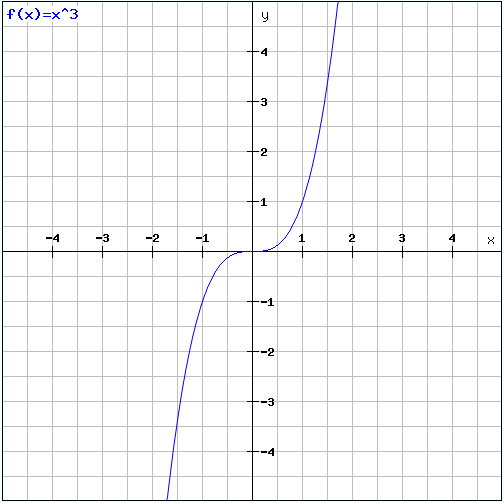
\includegraphics[width=0.35\textwidth]{Figures/f}
			\end{center}
	\end{figure}	
	
\end{frame}

%%%%%%%%%%%%%%%%%%%%%%%%%%%%%%%%%%%%%%%%%%%%%%%%%%%%%%%%%%%%%%%%%%%%%%%%%%%%%%%%%%%%%%%%%%
\subsection{Funções Bijetoras}

\begin{frame}
\frametitle{Funções}

	\begin{block}{Funções Bijetoras}
		\begin{itemize}
			\item Seja a função $h: A \to B$.
			\item $h$ é \textbf{bijetora} se é \textbf{injetora} e \textbf{sobrejetora}.
		\end{itemize}
	\end{block}
	
	\begin{figure}[!h]
			\begin{center}
			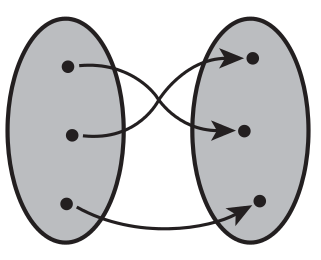
\includegraphics[width=0.5\textwidth]{Figures/bijetora}
			\end{center}
	\end{figure}	
	
\end{frame}


%%%%%%%%%%%%%%%%%%%%%%%%%%%%%%%%%%%%%%%%%%%%%%%%%%%%%%%%%%%%%%%%%%%%%%%%%%%%%%%%%%%%%%%%%%

\begin{frame}
\frametitle{Funções}

	\begin{block}{Funções Bijetoras}
		\begin{itemize}
			\item Seja a função $h: A \to B$.
			\item $h$ é \textbf{bijetora} se é \textbf{injetora} e \textbf{sobrejetora}.
		\end{itemize}
	\end{block}
	
	\begin{block}{Exemplo de uma Função Bijetora}
		\begin{itemize}
			\item Seja a função: $h: \mathbb{R} \to \mathbb{R} : h(x) = 2x$
		\end{itemize}
	\end{block}
	\begin{figure}[!h]
			\begin{center}
			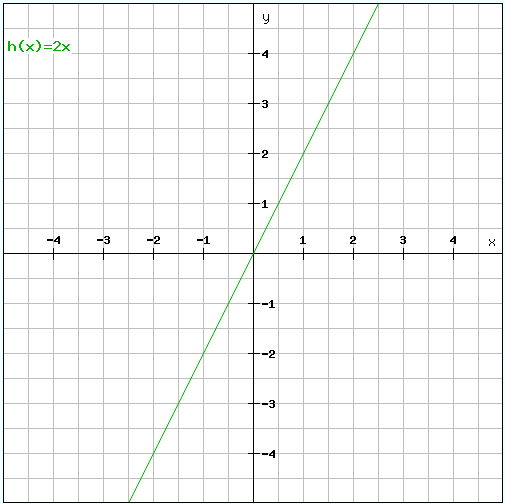
\includegraphics[width=0.35\textwidth]{Figures/h}
			\end{center}
	\end{figure}	
	
\end{frame}


%%%%%%%%%%%%%%%%%%%%%%%%%%%%%%%%%%%%%%%%%%%%%%%%%%%%%%%%%%%%%%%%%%%%%%%%%%%%%%%%%%%%%%%%%%
\subsection{Função Inversa}
\begin{frame}
\frametitle{Funções}

	\begin{block}{Funções Inversas}
		\begin{itemize}
			\item Seja a função $h : A \to B$.
			\item Definimos como função inversa de $h$, a função $h^{-1}: B \to A$ tal que: $ h \circ h^{-1} = id_x$ e $ h^{-1} \circ h = id_y$.
			\item $h(h^{-1}(x)) = x$ e $h^{-1}(h(x)) = y$
		\end{itemize}
	\end{block}
	
	\begin{figure}[!h]
			\begin{center}
			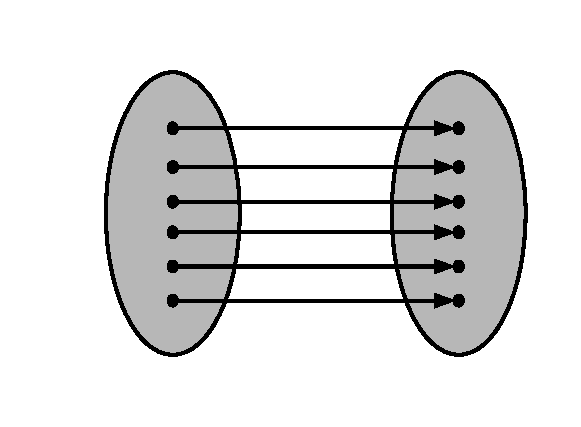
\includegraphics[width=0.6\textwidth]{Figures/inversa}
			\end{center}
	\end{figure}

\end{frame}

%%%%%%%%%%%%%%%%%%%%%%%%%%%%%%%%%%%%%%%%%%%%%%%%%%%%%%%%%%%%%%%%%%%%%%%%%%%%%%%%%%%%%%%%%%

\begin{frame}
\frametitle{Funções}

	\begin{block}{Funções Inversas}
		\begin{itemize}
			\item Seja a função $h : A \to B$.
			\item Definimos como função inversa de $h$, a função $h^{-1}: B \to A$ tal que: $ h \circ h^{-1} = id_x$ e $ h^{-1} \circ h = id_y$ tal que  $h(h^{-1}(x)) = x$ e $h^{-1}(h(x)) = y$
		\end{itemize}
	\end{block}
	
	\begin{block}{Exemplo de uma Função Inversa}
		\begin{itemize}
			\item Seja a função: $h: \mathbb{R} \to \mathbb{R} : h(x) = 2x$
		\end{itemize}
	\end{block}
	\begin{figure}[!h]
			\begin{center}
			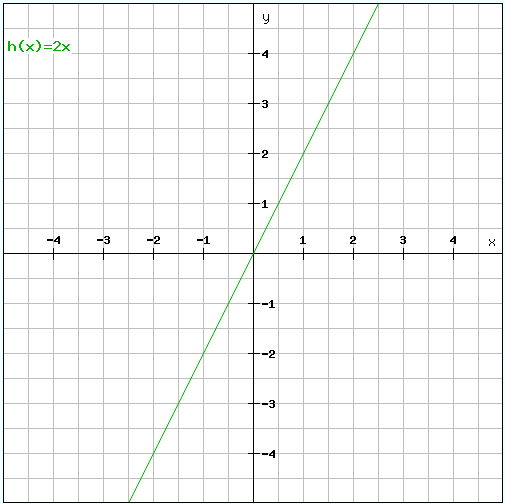
\includegraphics[width=0.25\textwidth]{Figures/h}
			\end{center}
	\end{figure}	
	
\end{frame}

%%%%%%%%%%%%%%%%%%%%%%%%%%%%%%%%%%%%%%%%%%%%%%%%%%%%%%%%%%%%%%%%%%%%%%%%%%%%%%%%%%%%%%%%%%

\begin{frame}
\frametitle{Funções}

	\begin{block}{Exemplo de uma Função Inversa}
		\begin{itemize}
			\item Seja a função: $h: \mathbb{R} \to \mathbb{R} : h(x) = 2x$
		\end{itemize}
	\end{block}
		\begin{eqnarray}
			h(x) = 2x \\
			h^{-1}(x) = \frac{y}{2} \\
			h(h^{-1}(x)) = 2(\frac{y}{2}) = y \\
			h^{-1}(h(x)) = \frac{2x}{2} = x
		\end{eqnarray}

\end{frame}







%----------------------------------------------------------------------------------------

\end{document} 